\section{Development Models}
There are many development models in the field that are inspired by nature. Though the concept of biological development does not change much, it is very much still a topic under discussion and there are still uncharted territories. It is therefore not surprising that these models differ not only in implementation, but also the biological ideas behind it. In this chapter, we will take a look at two models. We'll see how they work, and discuss their differences. These models are important for this thesis because they are believed to represent the greatest difference in development models to date.

\subsection{ArtDev3D}
\label{sec:Models:ArtDev3D}
In 2006, Johan H{\o}ye handed in his master's thesis\cite{hoye2006} based on his own model of biological development. Its aim was to draw inspiration from biology but simplify concepts to avoid dwelling too deep into the underlying and less understood concepts.

\subsubsection{Concepts}
To understand this model, we will have to touch a few topics in biology. Like with humans, everything starts out with a single cell, the zygote. The zygote divides and becomes two cells. These cells divide again to become four cells. This process repeats itself in a controlled fashion with the help of the DNA, the recipe of life. It tells which proteins to synthesize, how and when. The proteins, in turn, carry out all the actual work inside the cell. In his model, only four such tasks were defined:

\begin{itemize}
	\itemsep=0pt
	\item Change the type of the cell
	\item Regulate chemical levels
	\item ``Request'' cell division in several directions
	\item Synthesize/transcribe more proteins
\end{itemize}

I use ``request'' here because of the way this model works. The proteins queue a request for the cell to perform division in some directions. These requests are accumulated and if the stimuli levels are just right, it will be realized. Likewise, the proteins also request for a change of cell type. The proteins themselves need to be activated in order to request anything. This usually depends on the current chemical levels in the cell as well as nearby cells. The neighbourhood in this model is defined to be the cells that a cell are in direct contact with in free space. That is above, below, left, right, front and back. Six in total.

The cell is also ``programmed'' to perform a number of tasks independent of the DNA. Implemented functions include osmosis, or the exchange of chemicals (or hormones) with nearby cells, and performing the actual cell division in requested directions. This set of functions are fixed for every cell and is not changed through evolution like the DNA is.

\begin{figure}[!ht]
	\centering
	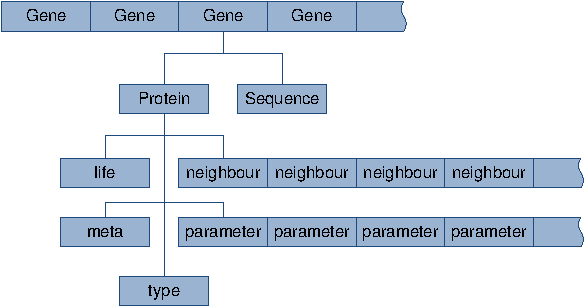
\includegraphics[scale=1.2]{artdev3d_genotype}
	\caption{Genotype representation in ArtDev3D}
	\label{fig:artdev3d_genotype}
\end{figure}

The genotype of this model (see fig~\ref{fig:artdev3d_genotype}), the DNA, is an array with genes. The genes carry a recipe for a protein and a genetic sequence. The gene sequence is used to find genes with desired proteins to synthesize. The protein type determines what its function is. If a protein that changes the cell's type is a type, then proteins that regulate chemicals are another. When the protein is activate is stored in the neighbours and chemicals array. The neighbours array stores the desired types of nearby cells. The chemicals array stores the desired chemical levels in the cell. When both of these are fulfilled, the protein is activated. Data in \texttt{meta} contain only one of two things, a cell type or a genetic sequence. These are used by the cell-type-changing and transcribing proteins respectively. The other two types only use the parameters. Figure~\ref{fig:artdev3d_protein-parameters} shows how the parameters are used to store the values to adjust the chemicals in a cell. Likewise, the proteins can store the directions it wants cells to divide into.

\begin{figure}[!ht]
	\centering
	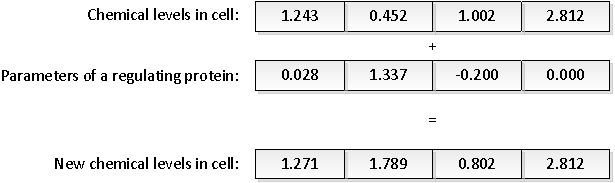
\includegraphics[scale=1.2]{artdev3d_protein-parameters}
	\caption{Parameters representation in ArtDev3D}
	\label{fig:artdev3d_protein-parameters}
\end{figure}

Any of these properties can be easily mutated and still be duplicated as a whole during cross over.

\subsubsection{How it works}
Development starts with an ``empty'' organism. The DNA is inserted into a cell before it is inserted to the organism. It becomes a zygote once the cell ``scans'' through the DNA and synthesizes all proteins. This is only performed in the initial cell. After initialization, the organism is developed by performing a set of operations on every cell every development step:

\begin{enumerate}
	\itemsep=0pt
	\item Determine activated proteins, usually by checking the internal chemical levels and neighbour cell types.
	\item All activated proteins request an action.
	\item Actions are accumulated, and executed. Depending on the action, the cell may regulate its chemical levels, synthesize proteins, change type, and perform cell division.
\end{enumerate}

Note that while the DNA indirectly requests actions upon the cell through the proteins, the cell performs the real work, like regulating the chemicals and proteins, behind the scene. The cell functions limit what the DNA can do, but at the same time, the DNA can affect both the cell and its surroundings using proteins as its proxy.

The development ends when a number of steps have passed, and the organism is rated based on how similar it is to the target phenotype. In this case, the targets are usually simple three-dimensional shapes.

While working with this model, it was discovered that the development algorithm does not develop all cells simultaneously. Usually, all cells must receive or gather information on nearby cells before any actions are executed. This is not the case here. Every cell gathers information and executes action in one go. So when the next cell gathers information, there will be ``new'' information mixed in. This flow is described in more detail in chapter~\ref{sec:Implementation:ArtDev3D}. However, the model seem to work rather well regardless. H{\o}ye's experiments also showed a number of interesting things. The initial number of don't-care-neighbours, i.e.\ the number of neighbours that can be of any type, had a negative impact on the growth of an organism when lowered. It was also shown that having a higher number of chemical types in the cells only contributed to making it harder to correctly develop the target shapes. This is most interesting because the next model we are going to discuss is based on chemicals, and it has been shown to work well.


\subsection{Artificial Development (ADCGP)}
Artificial development using Cartesian genetic programming is built on a genetic program invented by Julian Miller in 1998. The following description of what the model is and how it works is based on a number of articles, but mostly \cite{mteurogp2000} and \cite{ecal2003}. There may therefore be differences and inaccuracies when comparing to his latest work. The model is based on developing a feed-forward graph that maps an input to an output, or a digital circuit if you like.

\subsubsection{Concepts}
The model focuses a great deal on intercellular communication. In biology, this is achieved by means of secreting chemicals through the cell's membrane. The same membrane is also used to receive chemicals from other cells. Based on the presence of some chemicals, the cell performs a set of operations to see if a change in cell type is needed, and in which directions it should divide itself to.

\begin{figure}[!ht]
	\centering
	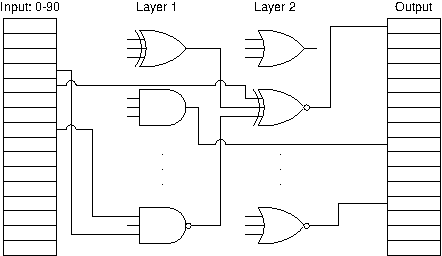
\includegraphics[scale=1.7]{cartesian_genotype}
	\caption{Genotype representation in artificial development}
	\label{fig:cartesian_genotype}
\end{figure}

The genotype of this model (fig.~\ref{fig:cartesian_genotype}) is a string of numbers that make up a feed forward circuit. This is represented as a set of four numbers where the first three points to a node, and the last number denotes which function to perform. The input to this function is the output of the nodes that the first three point to. We will see what this means in a moment.

In the simplified figure above (some gates aren't connected to avoid clutter), the input string consists of 90 bits, denoted 0 up to and including 89. Every gate, or node, are denoted 90-\emph{n}, where \emph{n} is the number of nodes. This means that the first gate we see in layer 1, is denoted 90, and the one under it is 91. Now we look at the genotype. As mentioned, it consists of four numbers. 7, 50, and 32 point to the corresponding bits in the input string, i.e.\ 7th, 50th and 32nd bits of the input string on the left. These bits are fed to the gate with a function identified by the fourth number. In this case, it is 10 - XOR. If an input number was higher than 89, it would be pointing to the output of a gate instead of the input string. The last few numbers of a genotype do not describe a circuit. They now point to either the input string or nodes. These bits make up the output string. There are no reason for why a node should be exactly four numbers. It can be any arbitrary number as long as it is consistent.

As opposed to ArtDev3D, every cellular activity is evolved. Nothing is programmed directly into the cell. Consequently, the evolved cell program can be difficult to analyze. The gates seen in figure~\ref{fig:cartesian_genotype} are just a series of Boolean operations.

\subsubsection{How it works}
There are several ways to start development with this model. One way is to represent the organism as a grid filled with cells and alternately give them maximum and no chemicals. The other way, and the way it is implemented here, is to start like ArtDev3D with a single cell and give it maximum chemicals. With the cell's and nearby cells' chemical levels, an input string is created and fed to the cell program. As the cell program is decided entirely by evolution (and chance), explanation of what happens inside the cell is nearly impossible. However, the end result is a string of numbers that determines whether or not the type of the cell should change and whether or not the cell should divide in a direction and how much chemicals the potentially new cell should be given.


\subsection{A generic development framework}
\label{sec:framework_requirements}
There are differences that can make it difficult to compare these two models. They differ not only in implementation but also in concepts and how they are represented. The most interesting thing to see here is that intercellular interactions in particular give different results in the two models.

In ADCGP, the cells communicate with each other using chemicals. The amount of chemicals exchanged, along with nearby cells' types determine what will occur in the cell in a development step. In ArtDev3D, communication happens without the chemicals. The state of the neighbourhood alone make up the external signals that contribute to determine whether or not some proteins are activated. Chemicals in ArtDev3D are used internally only and are not exchanged. Furthermore, it has shown that the number of chemical types is inversely related to fitness. Quite opposite of how ADCGP is reported to work. One can place these models on their own end of the scale. Because of this controversy, there are discussions as to whether chemicals really are necessary.

Moreover, there are other factors that come into play as well. For instance, the two models use different evolutionary algorithms, they evolve different genotypes, and the cell program is partly hard-coded in one model but not in the other. These are only two models in a relatively new field where a lot of research is still ongoing. How can we tell why something is working for one model, and not for the other? These kinds of questions can be difficult to answer with so many factors to consider.

To solve this problem, one can try and minimize the impact of these factors. This thesis proposes a framework that will provide a generic implementation of a development system that can embody any model without forcing compromises. Models that are implemented within this framework will share a common code base, making factors related to implementation and use of algorithms negligible. It will also become much clearer what one model uses or not, compared to another model.

Requirements for such a model should include:
\begin{itemize}
	\item\textbf{A genetic algorithm}

	Using a common genetic algorithm will eliminate discussions on whether or not a certain algorithm is better than another. The focus should be on the development model, and not genetic algorithms.

	\item\textbf{A development algorithm}

	Most of the models use the same basic algorithm for development, i.e.\ with every development step, every cell in an organism is told to execute their program. This occurs for a configurable number of steps, and varies very little from model to model. Hence, there is no need to implement this algorithm every time. In cases such as with ArtDev3D, this will automatically address the issue with simultaneous cell development as well.

	\item\textbf{A common messaging system}

	Especially with these two models, there are different things that go into a message that is sent to nearby cells. A common message should be able to contain most of a cell's properties while constrict the messages to just that and nothing more. The user can just choose the relevant parts for his or her model. When comparing, one should be able to say that two models differ because one uses chemicals while the other uses both chemicals and cell types.

	\item\textbf{Common concepts}

	It is important that a cell is always a cell, regardless of which model we are talking about. The definition of a cell should not change because a model wants it differently. Likewise, there should be only one definition for chemicals, organisms and proteins. While they are restricted and enforced on the user, it should also be generic enough to implement any model.

	\item\textbf{Protecting the organism}

	Access to the organism should be limited to avoid accidental tampering. Cell division will occur by telling the organism to add a cell in a particular location. This should be done through a function call. All information regarding the cellular neighbourhood should be available through the messaging system. As such, mechanisms should also be available to check whether a cell in a particular location exists or if it will be occupied by a new cell. This is to enable checks prior to performing cell division.
\end{itemize}

There are several benefits to using such a framework. First and foremost, it will cut down on implementation time. Such a model will allow a user to concentrate wholly on their model and not spend time implementing the most suitable genetic algorithm, or finding out whether or not the messaging system was implemented correctly. Instead, the user need only use what is already there and just fill in the blanks. Secondly, the implementation can be guaranteed to work. As the framework matures, the user can be assured that if something does not work, it is most likely their model and not because of a bug elsewhere in the system. Finally, and probably most importantly, the framework will hopefully be able to reduce the number of factors that prevent a clear verdict on a comparison.

We've seen that these two models are quite different from one another, which is why they will serve as an excellent starting point to implement the framework. One of the criteria for the framework is to be generic as it should be able to implement any model conceivable. It should also be able to perform at least as well as the original implementation did. We shall have a closer look at this in the next chapter.
